%% LaTeX2e class for student theses
%% sections/content.tex
%% 
%% Karlsruhe Institute of Technology
%% Institute for Program Structures and Data Organization
%% Chair for Software Design and Quality (SDQ)
%%
%% Dr.-Ing. Erik Burger
%% burger@kit.edu
%%
%% Version 1.1, 2014-11-21

%To be able to reference labels in other file
\externaldocument{introduction}
\externaldocument{appendix}

%%%%%%%%%%%%%%%%%%%%%%%%%%%%%%%%%%%%%%%%%%%%%%%%%%%%%%%%%%%%%%%%%%%%%
%--WATERTANK--%
%%%%%%%%%%%%%%%%%%%%%%%%%%%%%%%%%%%%%%%%%%%%%%%%%%%%%%%%%%%%%%%%%%%%%
\chapter{Motivating Example: Refinement of CPS ``Watertank''}
\label{ch:Watertank}

To better understand the process of refinement of a CPS we take an example from the \keym~tutorial~\cite{keYmaera}, a watertank (See Fig.~\ref{fig:watertank}) whose water level is adjusted automatically to stay at a certain level, and refine its hybrid model to gain an implementation. Our goal therefore is finding a suitable and verified implementation from the hybrid model with all necessary proof steps. To accomplish this, we have to adjust and verify the hybrid model, code and verify a concrete implementation and finally verify the ``glue'' in between the discrete and continuous world we come up with as our last proof steep. 

\begin{figure}[h!]
	\setcounter{figure}{0}
	\centering
	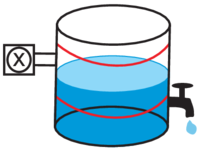
\includegraphics[width=0.6\textwidth]{images/watertank}
	\caption{Picture of possible Watertank configuration: Watertank that can get drained at all times and has a valve controlled by a control program~\cite{keymaeraGuide}.}
	\label{fig:watertank}
\end{figure}

The ``control'' part of this hybrid system is the valve, it can either drain the watertank with a rate of \(-2\) or it can fill the tank further with a rate of \(1\). The goal of the entire system then is, to keep the water level \(y\) of the tank between \(1\) and \(12\). Normally this is proven by \keym~ without actually implementing a control program. To be able to   we first took a look at the hybrid model of the watertank. It is provided both in the form of a hybrid automaton (See Fig.~\ref{fig:watertank_ha}) and a hybrid program (See sec.  \ref{pdf:watertank_hp}). In the hybrid automaton, the system starts in the ``fill'' state, where water is constantly flowing into the tank with the rate of \(y^{\prime} = 1\), while the clock is counting by \(x^{\prime}=1\) per tick. Once the water level reaches a certain level \(y=10\) the clock is reset to \(x:=0\) and the state changes from ``fill'' to ``stop'', where the water level is still raising for 2 ticks since the valve can not change in instant time. Once those 2 ticks pass \(x=2\) the watertank switches its state again to ``drain'' in which water flows out of the tank at the rate of 2 per clock tick, before it changes again to ``start'' the filling of the tank agan at the water level of \(y=5\).

\begin{figure}
	\centering
	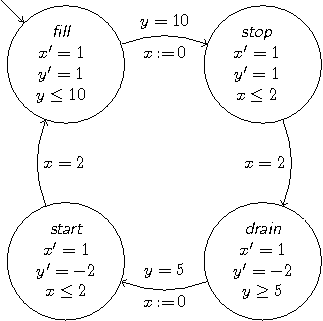
\includegraphics[width=0.6\textwidth]{images/watertank_ha}
	\caption{The Watertank CPS expressed as a hybrid automata~\cite{keymaeraGuide}.}
	\label{fig:watertank_ha}
\end{figure}

\phantomsection
\label{pdf:watertank_hp}
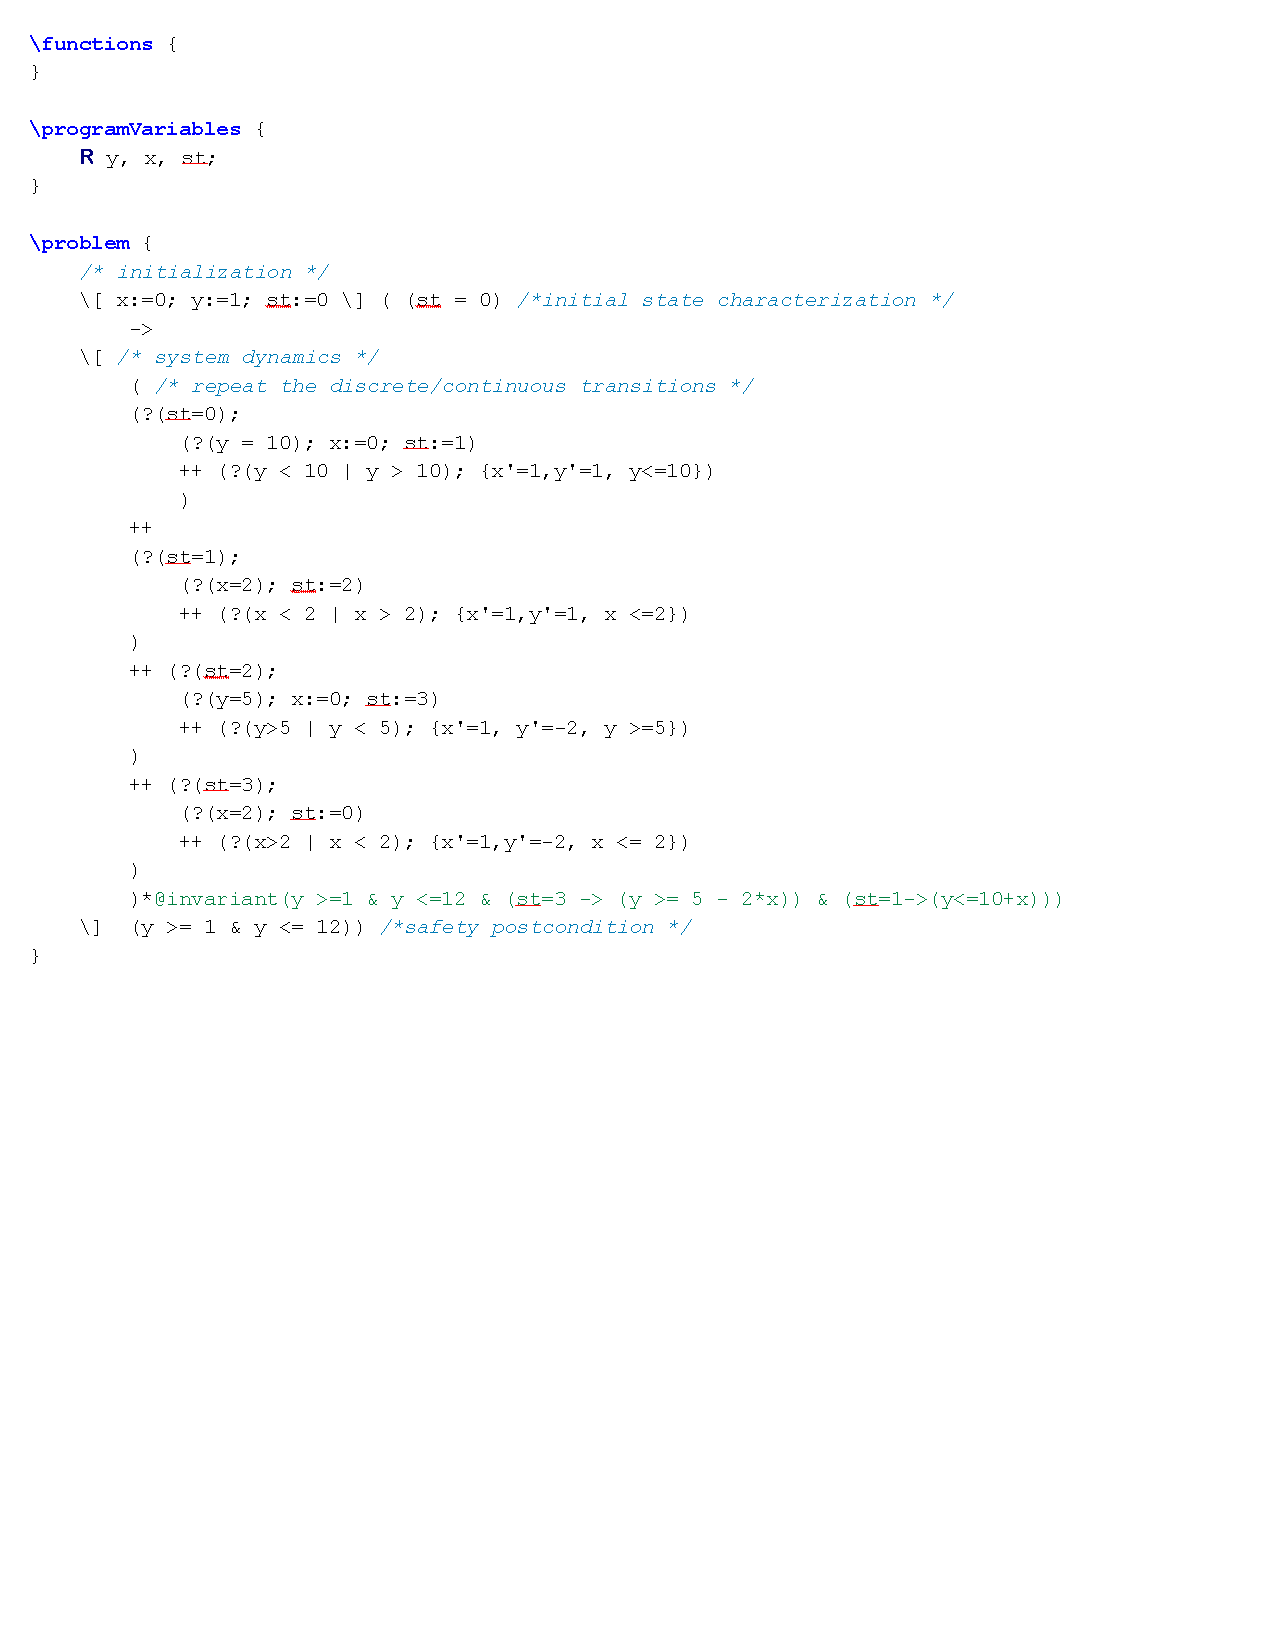
\includepdf[pages=1,scale=0.8]{images/watertank_hp.pdf}

\section{Finding the concrete Control Value Assisgnment}
\label{sec:Watertank:ControlValue}

In order to be able to apply Eq.~\ref{eq:Main_LogicRefinement} to this concrete example, we first found a spot in which a (or multiple) concrete control value is actually assigned. We call this assignment(s) the \textit{hook} as the actual implementation will ``hook'' into our hybrid model at this exact point. The Hybrid Automata describing the Watertank (See Fig.~\ref{fig:watertank_ha}), required changing to be able to find our actual ``hook''. In the original model, a control value is never explicitly assigned, rather does the valve change its state non-deterministically, making a deterministic control program implementation impossible, as the program can not act in a non-determnistic manner and would not fit in the model of the cps. Therefore, we remodelled the system to better serve our purpose, featuring a clear ticked hook that is called upon at deterministic times (See sec. \ref{pdf:watertank_hp_ref}).

\phantomsection
\label{pdf:watertank_hp_ref}
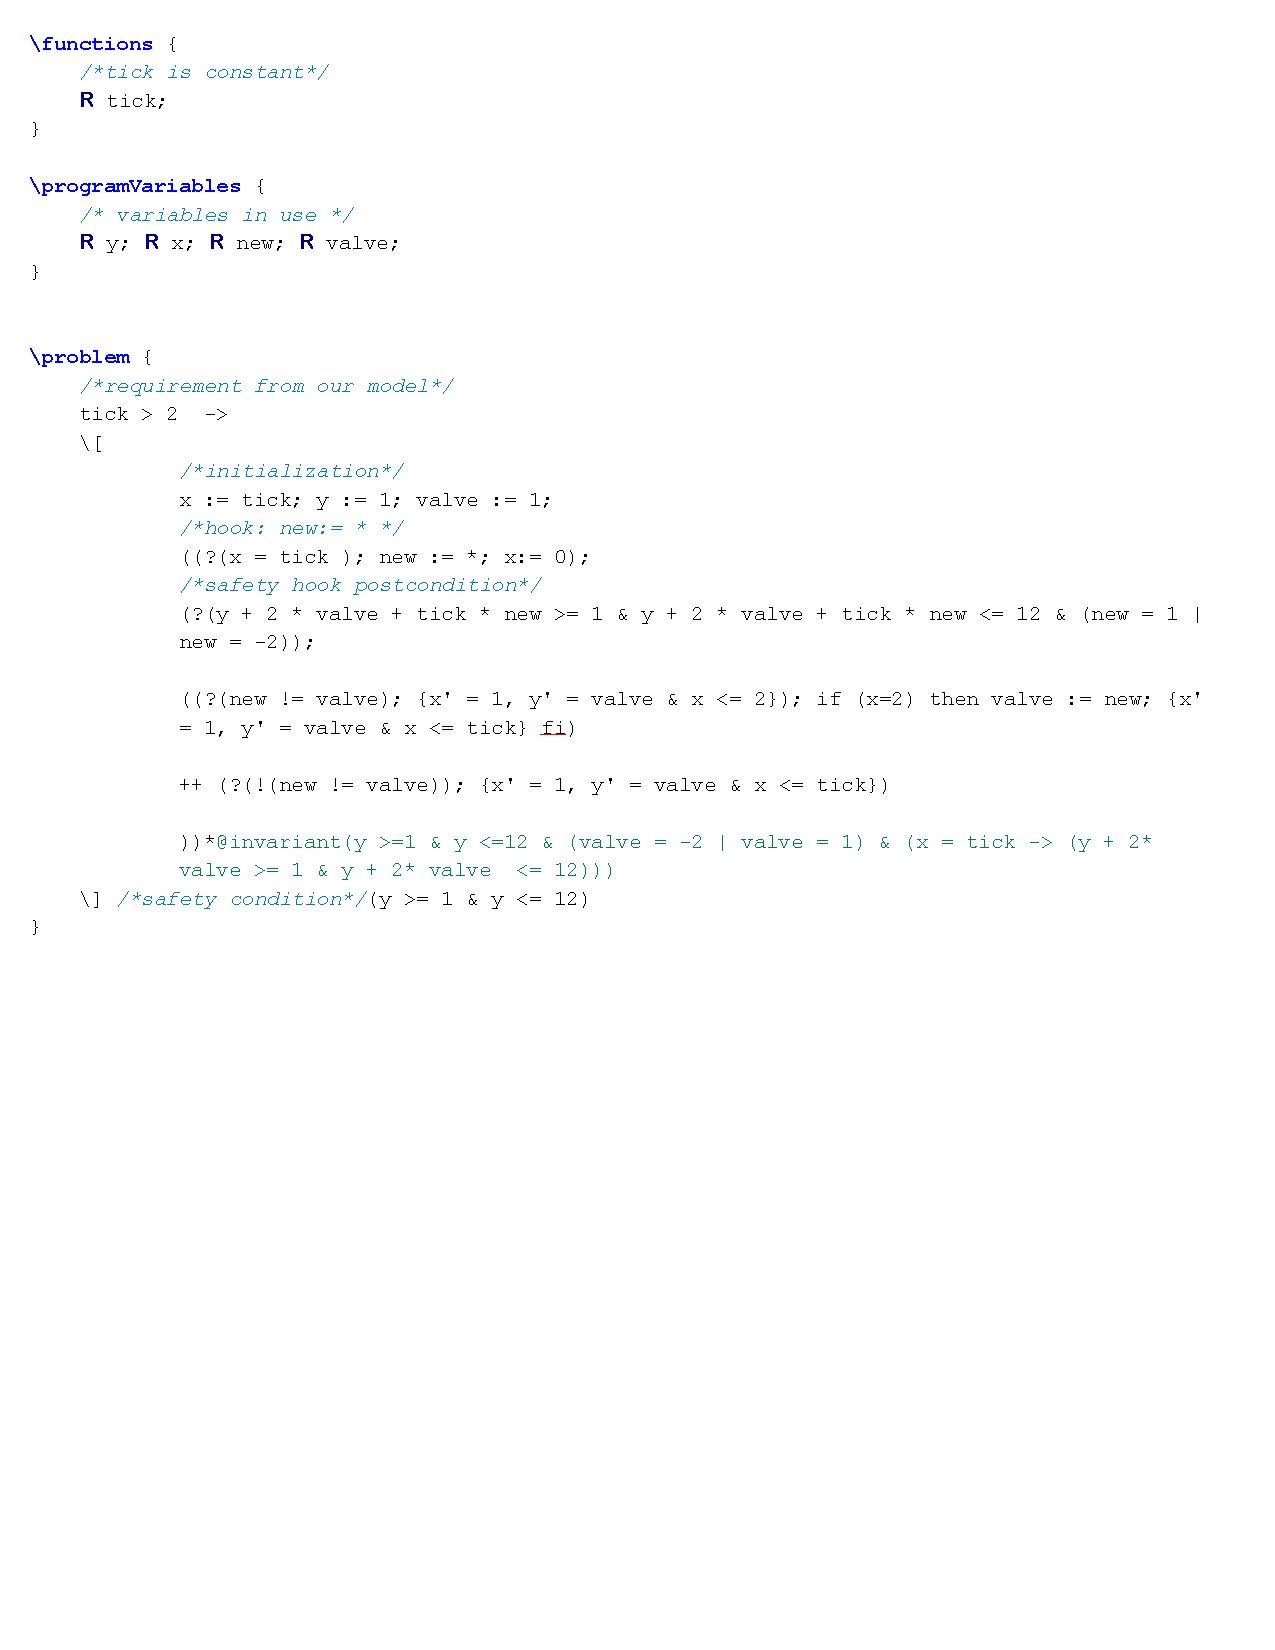
\includepdf[pages=1,scale=0.8]{images/Watertank.pdf}

We kept the model mostly equivalent to the original, preserving the two clock ticks of time needed for the valve to change its state from drain to fill and vice-versa. This presented a challenge, when thinking of possible implementations, as the program hook could be called again before the valve would have actually changed its state. To simplify this problem,we only model cases in which the actual program tick (so the time between two hook calls)  is greater than two clock ticks (however long they may be).  This means, that the valve or control program does not have to have a (possibly infinite) list of the last control values assigned, which could be the case if the program was called more frequently than the valve is able to change states.

\section{Finding the correct Program Safety Condition}
\label{sec:Watertank:SafetyCond}

Next we devised a postcondition for the program hook, which would then serve as the abstraction of the java control program implementation. This means, that the program would be built accordingly, so that it could be verified against this postcondition. The original postcondition we devised:

\begin{equation}
	\centering
	\begin{split}
		\psi \equiv (y + 2* valve + tick -2 * new  \geq 1 \wedge \\ 2 * valve * (tick - 2) * new \leq 12 \wedge \\  y + 2* valve \geq 1 \wedge  y + 2 * valve \leq 12) 
	\end{split}
\label{eq:postCondOrig}
\end{equation}

When trying to verify the entire hybrid program (see comment in line 5 of the problem in sec.~\ref{pdf:watertank_hp_ref}), this postcondition did not work. This means, that even in such a simple CPS as this watertank control system, finding the hook postcondition was non-trivial and only with the help of \keym's counterexamples did we manage to find the correct postcondition (See Eq.~\ref{eq:postCondOrigCorrect}). 

\begin{equation}
	\centering
	\begin{split}
		\psi \equiv (y + 2 * valve + tick * new \geq 1 \wedge\\ y + 2 * valve + tick * new \leq 12 \wedge \\(new = 1  \vee new = -2))
	\end{split}
	\label{eq:postCondOrigCorrect}
\end{equation}

\keym~ verified our new hybrid program fully automatically.

\section{The (simple) Java Control Program}
\label{sec:Watertank:Java}

After completing verification of our hybrid model with \keym, we proceeded to implement a (simple) control program for the Watertank. Finding a suitable implementation proved difficult, as a parallel implementation (Both the control system and the differential equations working in parallel, modifying the water level) seemed more intuitive. This would defeat the purpose of actually finding a suitable hook and was more based on our understanding of the original hybrid model and not our version including the hook.

Using our understanding of a singular hook of the control system into the watertank as well as the hook postcondition from the previous section as our specification for the actual control method, that would return the control value to the watertank's valve, we then managed to implement a suitable discrete control method (See Lst.~\ref{lst:source_controlMethod}).

\definecolor{darkgreen}{rgb}{0.0, 0.2, 0.13}
\lstset{language=Java,captionpos=b,tabsize=3,frame=lines,keywordstyle=\color{blue},commentstyle=\color{darkgreen},stringstyle=\color{red},numbers=left,numberstyle=\tiny,numbersep=5pt,breaklines=true,showstringspaces=false,basicstyle=\footnotesize,emph={label}}
\begin{lstlisting}[label=lst:source_controlMethod]
public int getControlValue (int y, int old) {
		//Waterlevel in two time units
		int inTwo = y + 2 * old;
		//If we are raising level, keep raising if possible without hitting max_level before next tick
		if (old == 10) {
			if (inTwo + tick * 1 <= 116) {
				return 10;
			}
			else {
					return -20;
			}
		}
		//ELSE if we are currently lowering level, keep lowering if we can lower further without hitting min_level b4 next tick
		else {
			if (old == -20) {
				if (inTwo - tick * 2 >= 12) {
					return -20;
				}
				else {
						return 10;
				
				}
		
			}
		}
		//Only returned if old != 10 && old != -20, unreachable.
		return 0;
}
}
\end{lstlisting}

The control method consists only of simple if-else-statements and just assigns the best-case (keep raising level if we were raising, keep lowering if we are lowering as long as postcondition is still valid) value to the valve. We translated the hook postcondition (See  Eq.~\ref{eq:postCondOrig}) into, what we thought to be, a suitable JDL postcondition statement for verification with \key~(See List.~\ref{lst:JDL}). In the next section we will explain why this postcondition would not work for our complete proof. \key~verified our program fully automatically, aside from the fact, that the \(tick>2\) precondition added too much computational complexity, so we let \key~prove the property with the more concrete \(tick==30;~tick==31;\dots\) assignments. 

For testing purposes, we also implemented a complete simulator of the Watertank CPS (See App.~\ref{app:Simulator}).

\begin{lstlisting}[label=lst:JDL]
	/*@ public normal_behavior //
	  @ requires tick == 30 && y >= 10 && y <= 120 && y + 2 * old <= 120 && y + 2 * old >= 10 && (old == 10 || old == -20); //
	  @ ensures \result * (tick / 10) + y + 2 * old  >= 12 & \result * (tick / 10) + y + 2 * old <= 116 && (\result == 10 || \result == -20); //
	  @*/
\end{lstlisting} 

\section{Finding the glue between Java and the Hybrid Model of the system}
\label{sec:Watertank:Glue}

As real values (used in the hybrid model) and discrete values (used in our java implementation) are fundamentally different, a certain transformation has to occur.  In the Watertank example, this means, that the waterlevel as well as the last valve-value (be it fill or drain), which are passed to the control method, have to be converted into one direction by the glue. 

Also, the result of the computation in the method (so the new valve value) has to be converted in the other direction. In general the glue is not necessarily a bijective function, as some values will not exist in both worlds, making it a relation. For the Watertank, fortunately, this problem doe not exist, so finding a function translating the waterlevel and valve values into each other instead of a relation simplifies the problem.

Finding the glue between the real parts of the hybrid system and our java control program still proved difficult though.

As we went along, we figured out how a general glue proof should look (See Fig.~\ref{eq:glueGeneral}). Here \(x\) are the discrete values in our control program, \(y\) are the real world values, \(\psi\) is the postcondition of the control program expressed using discrete values and \(\phi\) is the actual safety condition we want to show for the entire hybrid system.

\begin{equation}
	\centering
	\begin{split}
		\forall x \in (Discrete World)~\forall y \in (Real World):(x,y) \in \textit{glue} \implies (\psi(x) \implies \phi(y))
	\end{split}
	\label{eq:glueGeneral}
\end{equation}

Following this basic guideline, we were able to find a suitable glue relation (or in our case a bijective function) for this cps (See Eq.~\ref{eq:glueWatertank}).

\begin{equation}
	\begin{split}
		\forall y \in \mathbb{R} . \forall y_j \in \mathbb{Z}. \forall valve \in \mathbb{R}. \forall tick \in \mathbb{R}&. \forall tick_j \in \mathbb{Z} . \forall new \in \mathbb{Z}. \forall result \in \mathbb{R} : \\  [y_j = \textrm{floor}(10 * y)~\wedge&~ old_j = \textrm{floor}(10*valve) ~\wedge \\ tick_j = \textrm{floor}(10*tick)~\wedge&~result = 10 * new~\wedge \\ y >= 1~\wedge&~y \leq 12~\wedge \\ (valve = 1 ~\vee~valve = -2)~\wedge&~tick > 2] \implies \\  \{[result * tick_j/10 + y_j + 2 * old_j \leq 116~\wedge&~result * tick_j/10 + y_j + 2 * old_j \geq 12~\wedge \\ (result = 10~\vee&~result = -20)] \implies \\ y + 2 * valve + tick * new \geq 1~\wedge&~y + 2 * valve + tick * new \leq 12~\wedge \\ (new = 1~\vee&~new = -2)]\}
	\end{split}
	\label{eq:glueWatertank}
\end{equation}

As can be seen, the \(\psi(x)\) that we found for the glue is not equal to the original trivial postcondition for our java program (See List.~\ref{lst:JDL}). This can be explained by the floor functions that has to be used for translation from the \(\mathbb{R}\) into \(\mathbb{Z}\) world. Due to the usage of the floor function, we only can approximate the original value in the discrete world, and therefore these approximation erorrs have to be accounted for in \(\psi\). Again the fact that we only found this error in our original postcondition devised for the java program, proves the non-triviality of the process even in seemingly simple examples as this watertank.

\section{Verification based on \keym}
\label{sec:Watertank:Verification}

Verification of the glue proved difficult since \keym, or specifically Mathematica (\keym~backend algebraic solver), has problems with the translation of unintepreted functions. Therefore we found an abstraction of the floor function using inequalities to approximate it (See Eq.~\ref{eq:approxF}). 

\begin{align*}
		\forall x \in \mathbb{R^{+}}. \exists c \in \mathbb{R}. floor(x) = c \implies x-1 < c \wedge c \leq x \wedge c \geq 0
	\label{eq:approxF}
\end{align*}
Also, since \keym~does not deal with numbers outside of the reals, we generalized the preconditions for every variable to be in the reals. This obviously only strengthens the proof and therefore does not change the correctness.

This still lead to problems when using the automatic proof-mechanism, so we had to add a full new taclet fdef to the definition file to be able to use the automatic proover (See App..~\ref{app:lst:ruleF}).

Applying the rule manually to the floor function and changing the first-order-strategy (so the time at which quantifier elimination using mathematica is tried) from lazy (extending every possible leave with case differentiation) to eager (quantifier elimination as soon as possible), the proof runs automatically aside from the application of our own defined rule.

%%%%%%%%%%%%%%%%%%%%%%%%%%%%%%%%%%%%%%%%%%%%%%%%%%%%%%%%%%%%%%%%%%%%%
%--PROCESS--%
%%%%%%%%%%%%%%%%%%%%%%%%%%%%%%%%%%%%%%%%%%%%%%%%%%%%%%%%%%%%%%%%%%%%%
\chapter{Introduction of formalized approach of using refinement to gain a concrete implementation for a CPS}
\label{ch:Process}

What the Watertank example shows is the non-triviality of refining the hybrid model into an implementation and of the verification of all necessary parts. Overall it is obvious, that a formalized approach to the general problem presented in chapter~\ref{ch:Introduction} is necessary. In this chapter we present a possible formalized approach to the problem, that we deemed feasible.
\\


To aid readability we will now give an overview of the process without explanation, then detailing each step in the following sections. 

\begin{enumerate}
	\item Modelling CPS as Hybrid System that includes concrete hook.
	\item Finding the necessary safety condition of the control value for verification with \keym.
	\item Implementing control program according to (preiliminary) safety condition and Verification by \key.		
	\item Finding the correct ``glue'' between hybrid model and control program and its verification by \keym.
	\item Result validation: Does our implementation still match the correct safety condition after verifying the glue?
\end{enumerate}

Overall for verification of our resulting implementation three proof obligations exist:
\begin{enumerate}[label=\roman*]
	\item Proving correctness of our hybrid model that includes a hook and (probably) the hook postcondition with \keym.
	\item Proving correctness of our implementation according to the (preliminary) safety condition and verifiying it against it using \key.
	\item Proving correctness of our glue using \keym.
\end{enumerate} 

With correct verification of all three parts, we can deduce that Eq.~\ref{eq:Main_LogicRefinement} has been fullfilled and our goal has been reached.

\section{Modelling CPS as Hybrid System that includes concrete Hook}
\label{sec:Process:Hook}
Most CPS we took a look at (See \cite{keymaera} Tutorial, \cite[p.~5, p.~11]{platzer2010b} \dots) as examples, did not have a concrete spot in which a control program could ``hook'' in easily. This means, that the first step in our refinement process has to be finding a suitable hook for the control program, referring to one or more non-deterministic assignments of a/multiple control values. Mostly for already existing hybrid systems, as was the case in Sec.~\ref{sec:Watertank:ControlValue}, a complete changing of the model is necessary. When creating a new model, one should try to find a suitable spot for a non-deterministic control value assignment, and model a form of tick, so as to make an implementation actually feasible.

To prevent issues in later verification of the model, a hybrid program and not a hybrid automata representation of the model should be chosen (cf.~\cite[ch.~1.1.4]{platzer2010b}). Since the modelling of the system can often be incorrect and a formal way to verify if the model correctly models all necessities does not exist, great care should be enacted during modelling of the cps.

\section{Finding the necessary safety condition of the control value for verification with \keym}
\label{sec:Process:SafetyCond}

After finding a suitable hook spot in our program we have the analyze the hook for a safety condition. If we think back to the watertank example (See ch.~\ref{ch:Watertank:SafetyCond}), this was non-trivial as the first postcondition we came up with through logic deduction proved to be incorrect. When thinking of possible conditions we often found we overlooked the tick when considering different postconditions. Obviously, more than one valid postcondition exists, as the constraints imposed on the implementation can get arbirtrarily strong and we're not restricting the actual behavior of the physical part of the cps. 

One should try and find the most general postcondition \(\psi\) for which the safety condition still holds, as this makes it easier to code the actual implementation with less constraints. Of course, if the model's proof works without any postcondition, this means that the program could also just assign random values making the implementation and glue trivial or non-existant. With correct modelling and sufficiently complex hybrid system (which even the relatively easy watertank had) this should never occur though.

The entire hybrid model with the hook safety postcondition should then be verified by \keym.

\section{Implementing control program according to safety condition as its specification and verification by \key.}
\label{sec:Process:Implementation}

Implementation of the program can theorethically be done in any preferred language, for usage with \key~as the automatic prover, Java is preferred. The implementation is free from any constraints asides from the postcondition that was devised previously, and from the constraints provided by \key~itself (No threading etc.). Since the postcondition is in the hybrid model and therefore written in the form of real variables and values, one has to already think of a form of the glue that will be formally devised as the next step, as to find a suitable translation of the postcondition expressed with real values into JDL. This can be a preliminary condition, as it is possible (as in Sec.~\ref{sec:Watertank:Glue}) that the formal glue will show errors in the original safety condition.

The implementation with its postcondition expressed in JDL then has to be verified by \key~before continuing with the glue. 

\section{Finding the correct glue between hybrid model and control program and verifying it with \keym.}
\label{sec:Process:Glue}

As both our model and implementation are now verified, the actual glue between the implementation and the model has to be devised. In the previous Chapter we came up with a general definition of what the glue relation provides:

\begin{equation}
	\centering
	\begin{split}
		\forall x \in (Discrete World)~\forall y \in (Real World):(x,y) \in \textit{glue} \implies (\psi(x) \implies \phi(y))
	\end{split}
	\tag{\ref{eq:glueGeneral}}
\end{equation}

Coming up with the glue is the hardest part of the entire process, and for us took multiple iterations before a correct and verified glue was found. Most of the time the glue will probably incorporate some form of rounding/flooring mechanism, as we have to translate real values into discrete ones. This makes the entire proof hard to fully understand without lots of complex mathematical computations, making the proof hard for humans.

We used a form of logical deduction to come up with the correct quantifiers for the glue proof (so the \(\forall\) in Eq.~\ref{eq:glueGeneral}), which can be found in App.~\ref{app:glueQuant}. Verification of the glue should then happen using \keym, which means formulation of the glue should already be in the required syntax of DDL.

Overall this means, that for the discrete-world postcondition \(\psi\) that was proven by \key~ and the real-world postcondition \(\phi\) that we came up with in step 3, and the glue that we devise which is verified by \keym, we reach the goal we set out for (See Eq.~\ref{eq:Main_LogicRefinement}).

\section{Validating glue results against implementation}
\label{sec:Process:Eval}

As we realized in our Watertank example (See Sec.~\ref{sec:Watertank:Glue}), with verification of our glue some changes might have to be made to the implementation and its postcondition. To complete the process of refinement we have to change the implementation and JDL condition and verify it again with \key~, make sure all our decisions made were actually valid and correct when taking a look back at the entire picture according to Eq.~\ref{eq:Main_LogicRefinement}).


%% -------------------
%% | Example content |
%% -------------------
\iffalse
The content chapters of your thesis should of course be renamed. How many
chapters you need to write depends on your thesis and cannot be said in general.

Check out the examples theses in the SDQWiki:

\url{https://sdqweb.ipd.kit.edu/wiki/Abschlussarbeit/Studienarbeit}

Of course, you can split this .tex file into several files if you prefer. 


\section{First Section}
\label{sec:FirstContent:FirstSection}

\dots

\section{Second Section}
\label{sec:FirstContent:SecondSection}

\dots


\chapter{Second Content Chapter}
\label{ch:SecondContent}

\dots

\section{First Section}
\label{sec:SecondContent:FirstSection}

\dots

\section{Second Section}
\label{sec:SecondContent:SecondSection}

\dots

Add additional content chapters if required by adding new .tex files in the
\code{sections/} directory and adding an appropriate 
\code{\textbackslash include} statement in \code{thesis.tex}. 
\fi
%% ---------------------
%% | / Example content |
%% ---------------------